\title{CS 472 HW 3}
\author{
        Aaron Havens \\
}
\date{\today}

\documentclass[12pt]{article}
\usepackage{amssymb} %maths
\usepackage{amsmath} %maths
\usepackage{graphicx}
\graphicspath{{figs/}}
\usepackage{qtree}
\begin{document}
\maketitle

\section{Problem 3.26, Russel}
Consider the unbounded version of the regular 2D grid shown in Figure 3.9. The start
state is at the origin, (0,0), and the goal state is at (x, y).
\paragraph{a) What is the branching factor b in this state space?}
The branching factor is \underline{\textbf{4}} for this discrete 2D state-space.
\paragraph{b) How many distinct states are there at depth k (for k $>$ 0)?}
When considering the number distinct states at any given depth k, we only think about the states that are reachable from a depth $k-1$ and haven't been previously visited by any other expansion. In this case the states expand along the ``perimeter'' of the graph as function of $\underline{\textbf{4k}}$.
\begin{figure}[ht]
\begin{center}
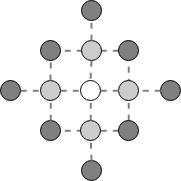
\includegraphics[scale=.65]{part_a}
\caption{Shown is an expansion of depth 2 in the 2D state space mentioned. The colors indicate the distinct states for each expansion.}
\end{center}
\end{figure}
\paragraph{c) What is the maximum number of nodes expanded by breadth-first tree search?}
A a tree search, the program has no memory of previously reached nodes by any other expansion. Therefore it follows the branching factor of $b = 4$ as $4^k$. However, depending on how BFS is implemented, depth of expansion may vary. If you expand at each node and then check that node for a solution, you must expand to a depth of k, but if you check for a solution before expanding that node, you need only $k-1$ depths. If you want to represent the number of expansions at some depth in terms of your goal (x,y), the following expression may be used.
\begin{align}
k = |x| + |y| \quad \text{or} \quad k = |x| + |y| -1\\
n = 4^{|x| + |y|} \quad \text{or} \quad 4^{|x| + |y| -1}
\end{align}
\begin{figure}[ht]
\begin{center}
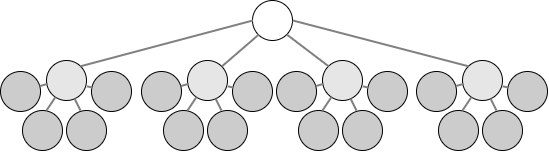
\includegraphics[scale=.65]{part_c}
\caption{The tree expansion of the 2D state space represented by a branching factor of 4. Nodes are colored by depth in which BFS would visit.}
\end{center}
\end{figure}
However, we want total number of nodes expanded which we would be the result of the sum of exponential expansion expressions fro 1 to k depth. Using the case where we check for solution before expanding results in the follow expression using a finite geometric series sum.
\begin{align}
\sum_{i=0}^{n} 4^i = \frac{4^{n+1}-1}{3}
\end{align}
Now representing depth in terms of our goal state (x,y), counting the root node expansion...
\begin{align}
n = \sum_{k=0}^{|x|+|y| - 1} 4^k= \frac{4^{|x|+|y|}-1}{3} \quad \text{where depth is k+1}
\end{align}
\paragraph{d) What is the maximum number of nodes expanded by breadth-first graph search?}
The maximum number of expanded nodes for graph is the total number of distinct states expanded summed over every depth expansion. We can calculate this number by summing over the expression in part b under the case of checking node solutions before expanding them.
\begin{align}
\begin{split}
n = 1 + \sum_{k=1}^{|x|+|y|-1} 4k =1 + 4(1) + 4(2) + ...+4(|x|+|y|-1) \\
= 1 + 4(1 + 2 + ... + (|x|+|y| -1))\\
= 1 + 2(|x|+|y|-1)(|x|+|y|)\\
as \quad k \rightarrow \infty \quad n \approx 2k^2.
\end{split}
\end{align}
\paragraph{e) Is $h = |u - x| + |v - y|$ an admissible heuristic for a state at (u, v)? Explain.}
Yes, the path to the goal will always be exactly or greater than the heuristic value in a 2D grid environment. There is no over estimation of the cost to the goal. This happens to be called the \textit{Manhattan Distance}.
\paragraph{f) How many nodes are expanded by $A^{\star}$ graph search using h?}
The heuristic makes it so that any distinct expansion in the quadrant of the goal has an equal cost. Therefore we will expand every node in the goal's quadrant bounded by (0,0) and (x,y). This number is \textbf{exactly $|xy|-1$} in the worst case (checking goal before expanding, counting the origin state).
\paragraph{g) Does h remain admissible if some links are removed?}
Yes. If any path are removed from the grid, a solution along that path can only be longer than before. Therefore there is still no overestimation of cost.
\paragraph{h) Does h remain admissible if some links are added between nonadjacent states?}
This violates the overestimation constraint. Any links to non-adjacent states allows one to ``cut corners'' or jump to any point on the grid. There would be cases in which the Manhattan distance overestimates the shortest path. In figure 3-b it shows a link that would make path cost 3 due to the diagonal connection, but the heuristic would compute $J = 1 + h(x) = 4$.
\begin{figure}[ht]
\begin{center}
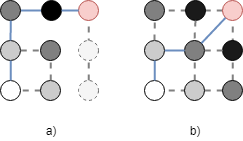
\includegraphics[scale=.8]{part_e}
\caption{\textit{a} describes a graph in which links are missing, but the Manhattan distance heuristic is still admissible, where \textit{b} would overestimate the shortest path given a non-adjacent link.}
\end{center}
\end{figure}
\end{document}